\documentclass[tikz,border=5pt]{standalone}
\usepackage{amssymb}
\usepackage{amsfonts}
\usepackage{mathrsfs}
\usepackage{amsthm}
\usepackage{amsmath}
\usepackage{xcolor}
\usepackage{hyperref}
\usepackage{libertinus}
\usepackage{dsfont}
\usepackage{bm}
\usepackage{enumitem}
\usepackage{caption}
\usepackage{subcaption}
\usepackage{tikz}
\usepackage{quiver}

\newcommand{\R}{\mathbb{R}}
\newcommand{\C}{\mathbb{C}}
\newcommand{\N}{\mathbb{N}}
\newcommand{\Z}{\mathbb{Z}}
\newcommand{\Q}{\mathbb{Q}}

\newcommand{\id}{\operatorname{id}}

% differentials and derivatives
\renewcommand{\d}{\mathrm{d}}
\newcommand{\dd}{\,\d}
\newcommand{\pddf}[2]{\frac{\partial#1}{\partial#2}}
\newcommand{\ddt}{\frac{\d }{\d t}}
\newcommand{\ddtz}{\left.\ddt\right|_{t=0}}

\begin{document}
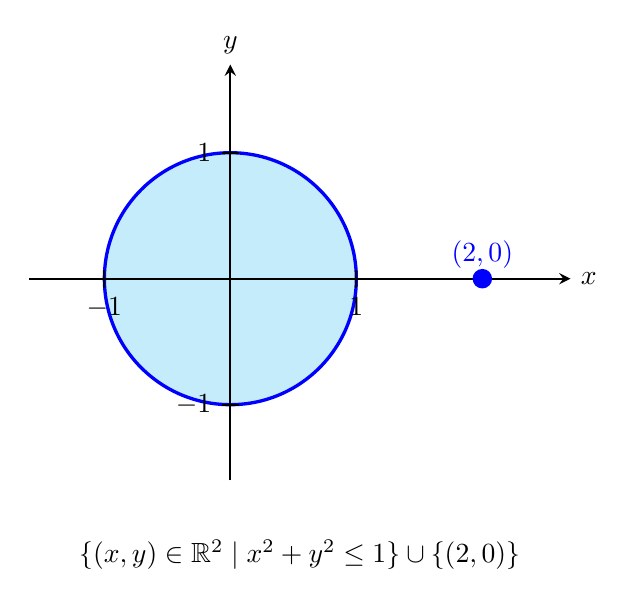
\begin{tikzpicture}[scale=1.6, >=stealth]

    % The closed unit disk
    \fill[cyan!45, opacity=0.5] (0,0) circle (1);
    \draw[blue, very thick] (0,0) circle (1);

    % Axes
    \draw[->, thick] (-1.6,0) -- (2.7,0) node[right] {$x$};
    \draw[->, thick] (0,-1.6) -- (0,1.7) node[above] {$y$};

    % Unit ticks
    \draw[thick] (1,0.07) -- (1,-0.07) node[anchor=north] {$1$};
    \draw[thick] (-1,0.07) -- (-1,-0.07) node[anchor=north] {$-1$};
    \draw[thick] (0.07,1) -- (-0.07,1) node[anchor=east] {$1$};
    \draw[thick] (0.07,-1) -- (-0.07,-1) node[anchor=east] {$-1$};

    % The isolated point, at distance 1 from the disk
    \fill[blue] (2,0) circle (2.2pt) node[anchor=south] {$(2,0)$};

    % \node[blue, anchor=north east] at (-0.72,-0.72) {$x^2+y^2=1$};

    \node[anchor=north] at (0.55,-2)
        {$\{(x,y)\in\R^2 \mid x^2+y^2\leq 1\}\cup\{(2,0)\}$};

\end{tikzpicture}
\end{document}
